\chapter{Introduction}

\section{Artificial Intelligence}

% Artificial Intelligence is a branch of Computer Science concerned with the study and creation of computer systems that exhibit some form of intelligence.
% \begin{enumerate}[label=\alph*.]
%     \item Learn new concepts
%     \item Reason and draw useful conclusions about the world
%     \item Understand a natural language or perceive and comprehend a visual scene
%     \item Perform other types of feats that require human types of intelligence
% \end{enumerate}

% From the perspective of Peter Norvig and Stuart Russell, AI definitions are organized along two dimensions. The definitions on top are concerned with thought processes and reasoning, whereas the ones on the bottom address behavior. The definitions on the left measure success in terms of fidelity to human performance, whereas the ones on the right measure against an ideal performance measure, called rationality.

From the perspective of Peter Norvig and Stuart Russell, AI definitions are organized along two dimensions. Definitions on top focus on thought processes and reasoning, while those on the bottom address behavior. Definitions on the left measure success by fidelity to human performance, whereas those on the right measure against an ideal performance called rationality.

\begin{center}
   \begin{tabular}{c|c}
      Thinking Humanly & Thinking Rationally \\\hline
      Acting Humanly & Acting Rationally
   \end{tabular}
\end{center}


\section{Tree Structure of AI Sub-fields}

The field of Artificial Intelligence (AI) is broad and consists of several sub-fields. The following tree structure illustrates the main sub-fields of AI and their relationships:

\begin{center}
\begin{tikzpicture}[
  level 1/.style={sibling distance=70mm},
  level 2/.style={sibling distance=40mm},
  level 3/.style={sibling distance=20mm},
  edge from parent/.style={draw,-latex},
  every node/.style={font=\small, align=center, anchor=north}
  ]

  \node (AI) {Artificial Intelligence}
   child {node (Symbolic) {Symbolic\\Learning}
      child {node {Computer\\Vision}}
      child {node {Robotics}}
   }
   child {node (ML) {Machine\\Learning}
      child {node {Statistical\\Learning}
         child {node {Speech\\Recognition}}
         child {node {NLP}}
      }
      child {node (DL) {Deep\\Learning}
         child {node {CNN} child {node {Computer\\Vision} child {node {Object Detection}}}}
         child {node {RNN}}
      }
   };

  \node[above left = 0.75cm and 0 of Symbolic] (ImageProc) {Image\\Processing};
  \draw[->, dashed, thick, orange, bend right=20] (ImageProc) to (Symbolic.north west);

  \node[above right = 0.75cm and 0 of ML] (PR) {Pattern\\Recognition};
  \draw[->, dashed, thick, orange, bend left=20] (PR) to (ML.north east);

  \node[above right = 0.5cm and 0 of DL] (NN) {NN};
  \draw[->, dashed, thick, orange, bend left=20] (NN) to (DL.north east);

  \node[below right = 0.1cm and 7 of AI] (SL) {Supervised\\Learning};
  \node[below = 1 of SL] (UL) {Unsupervised\\Learning};
  \node[below = 3 of UL] {Reinforcement\\Learning};

\end{tikzpicture}
\end{center}

\section{Comparison between AI, ML and DL}
\begin{tabularx}{\textwidth}{|l|L|L|L|}\hline
   \textbf{Aspect} & \textbf{Artificial Intelligence} &
   \textbf{Machine Learning} & \textbf{Deep Learning} \\\hline
   
   Definition
   & AI simulates human intelligence to perform tasks and make decisions.
   & ML is a subset of AI that uses algorithms to learn patterns from data.
   & DL is a subset of ML that uses artificial neural networks for complex tasks.
   \\\hline
   
   Goal 
   & Make machines smart and mimic human reasoning.
   & Enable machines to learn patterns from data.
   & Automate feature extraction and complex pattern learning.
   \\\hline
   
   Data Dependency
   & Can work with rules or data
   & Requires structured data for training
   & Requires large amounts of data for high performance
   \\\hline
   
   Algorithms
   & Expert systems, search, logic, decision trees
   & Regression, classification, clustering
   & CNN, RNN, Transformers
   \\\hline
\end{tabularx}


% Explain an Al Expert System with its three basic building blocks and necessary diagram.

\section{Al Expert System}
Expert systems are knowledge-based systems which contain expert knowledge and can provide an expertise, similar to the one provided by an expert in a restricted application area.

An expert system consists of the following main blocks:
\begin{itemize}[parsep=0.5em, topsep=-0.5em]
   \item Knowledge base (data base)
   \item Inference engine (explanation module)
   \item User interface (knowledge acquisition module)
\end{itemize}



\begin{figure}[h!]
   \centering
   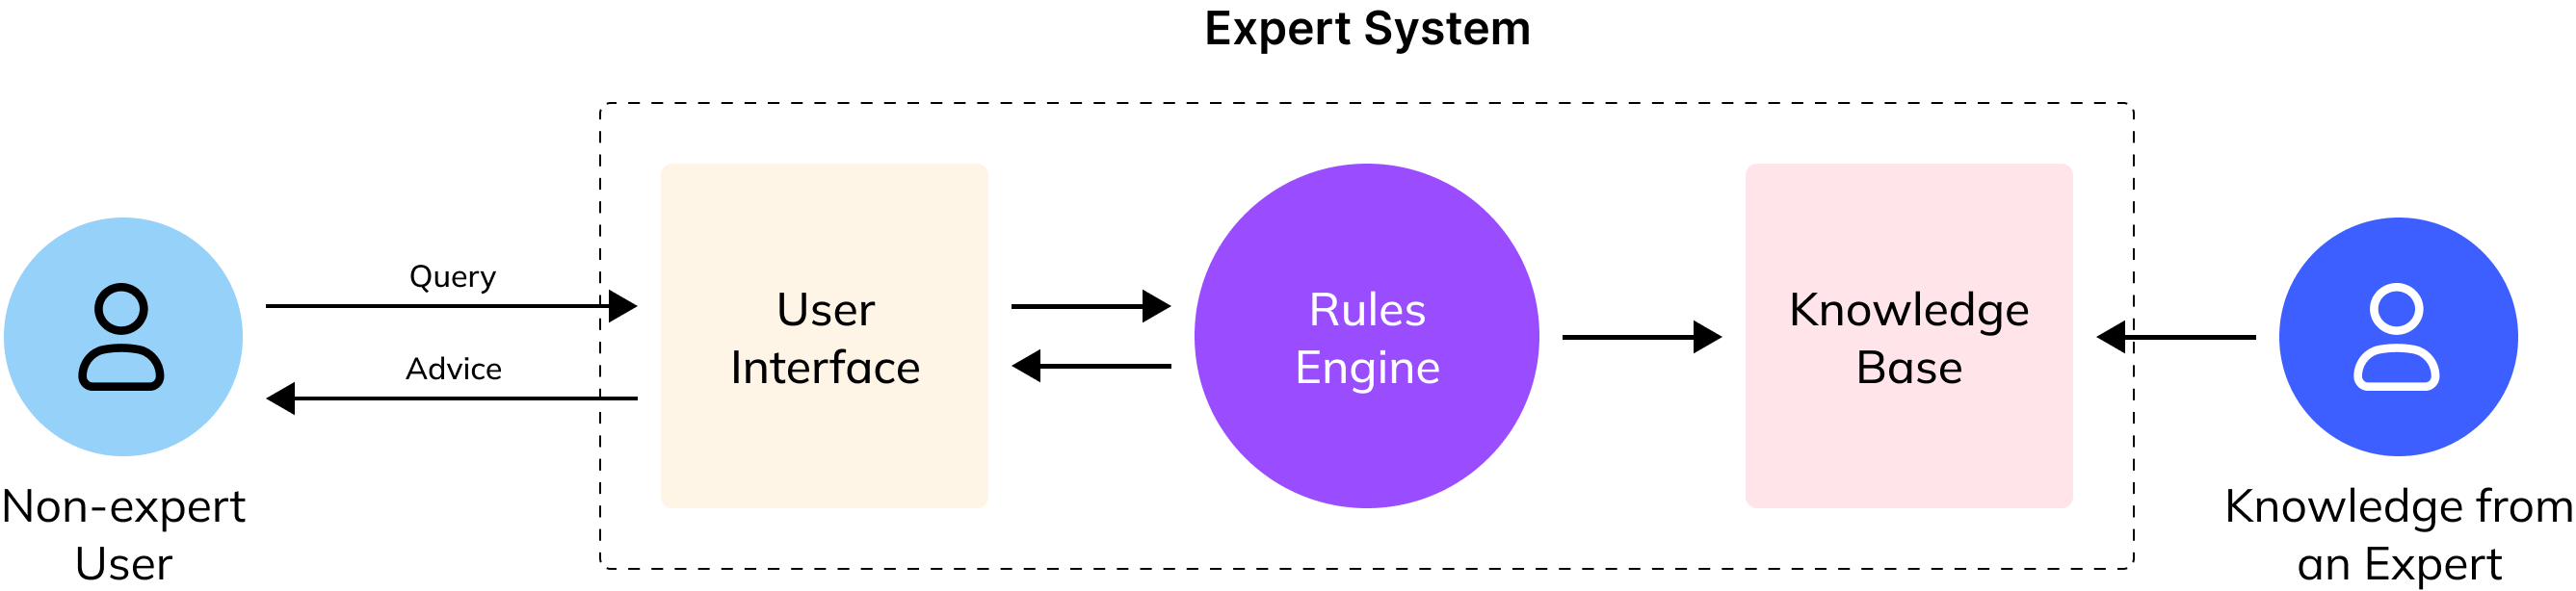
\includegraphics[width=0.7\textwidth]{figures/Expert System.png}
   \label{fig:expert-system}
\end{figure}

% Al is different from Machine Learning and Deep Learning. Justify your answer with [4)
% your own logic.
% In an automated CPU design company, ensuring that only defect-free CPUs move forward in the production line. Detecting defective CPUs manually from thousands of CPUs daily, is impractical and time-consuming for human. To enhance efficiency, an Al-powered system can be implemented to inspect and classify CPUs based on defects, performance metrics, and manufacturing accuracy. Analyze the PEAS properties of a "CPU Defect Detection Agent."

\section{Turing Test}

The Turing Test, proposed by Alan Turing (1950), evaluates a machine's intelligence. A computer passes the test if a human interrogator, after posing some written questions, cannot tell whether the written responses come from a person or from a computer.

\textbf{Capabilities required to pass the Turing Test:}
\begin{itemize}[parsep=0.5em]
   \item Natural language processing - to communicate fluently in human language.
   \item Automated reasoning - to use the stored information to answer
   questions logically.
   \item Knowledge representation - to store what it knows or hears
   \item Machine learning - to adapt to new circumstances and recognize patterns.
\end{itemize}

\textbf{Additional capabilities to pass the Total Turing Test:}
\begin{itemize}[parsep=0.5em]
   \item Computer vision - to perceive and understand visual input.
   \item Robotics / Physical interaction - to manipulate objects and interact with the environment.
\end{itemize}

% The Turing Test, proposed by Alan Turing in 1950, evaluates whether a machine can exhibit intelligent behavior indistinguishable from that of a human. A computer passes the test if a human interrogator, through written conversation, cannot reliably tell whether the responses come from a human or a machine.

% The Turing Test is a concept in artificial intelligence proposed by Alan Turing in 1950 to evaluate a machine's ability to exhibit intelligent behavior indistinguishable from that of a human.

% A computer passes the test if a human interrogator, after posing some written questions, cannot tell whether the written responses come from a person or from a computer. The machine must use natural language, reason, have knowledge and learn.

% The test can be extended to include video input, as well as a "hatch" through which objects can be passed: this would force the machine to demonstrate skilled use of well designed vision and robotics as well.

% The "Total Turing Test" is an expansion of the original Turing Test that includes visual and physical tasks, requiring a machine to demonstrate not only human-like conversation but also human-like perception and physical interaction through its ability to see, understand the physical world, and manipulate objects.